\documentclass[final]{beamer}
\mode<presentation>
{
  \usetheme{collis} 
}
\graphicspath{{figures/}}

\usepackage{times}
\usepackage{amsmath,amssymb}
\usepackage[english]{babel}
\usepackage[latin1]{inputenc}
\usepackage[printwatermark]{xwatermark}
\usepackage[orientation=landscape,size=a0]{beamerposter}  % e.g. custom size poster
\usepackage{tikz}
\addtobeamertemplate{block begin}{\pgfsetfillopacity{0.8}}{\pgfsetfillopacity{1}}


\usebackgroundtemplate{
\tikz\node[opacity=0.5] {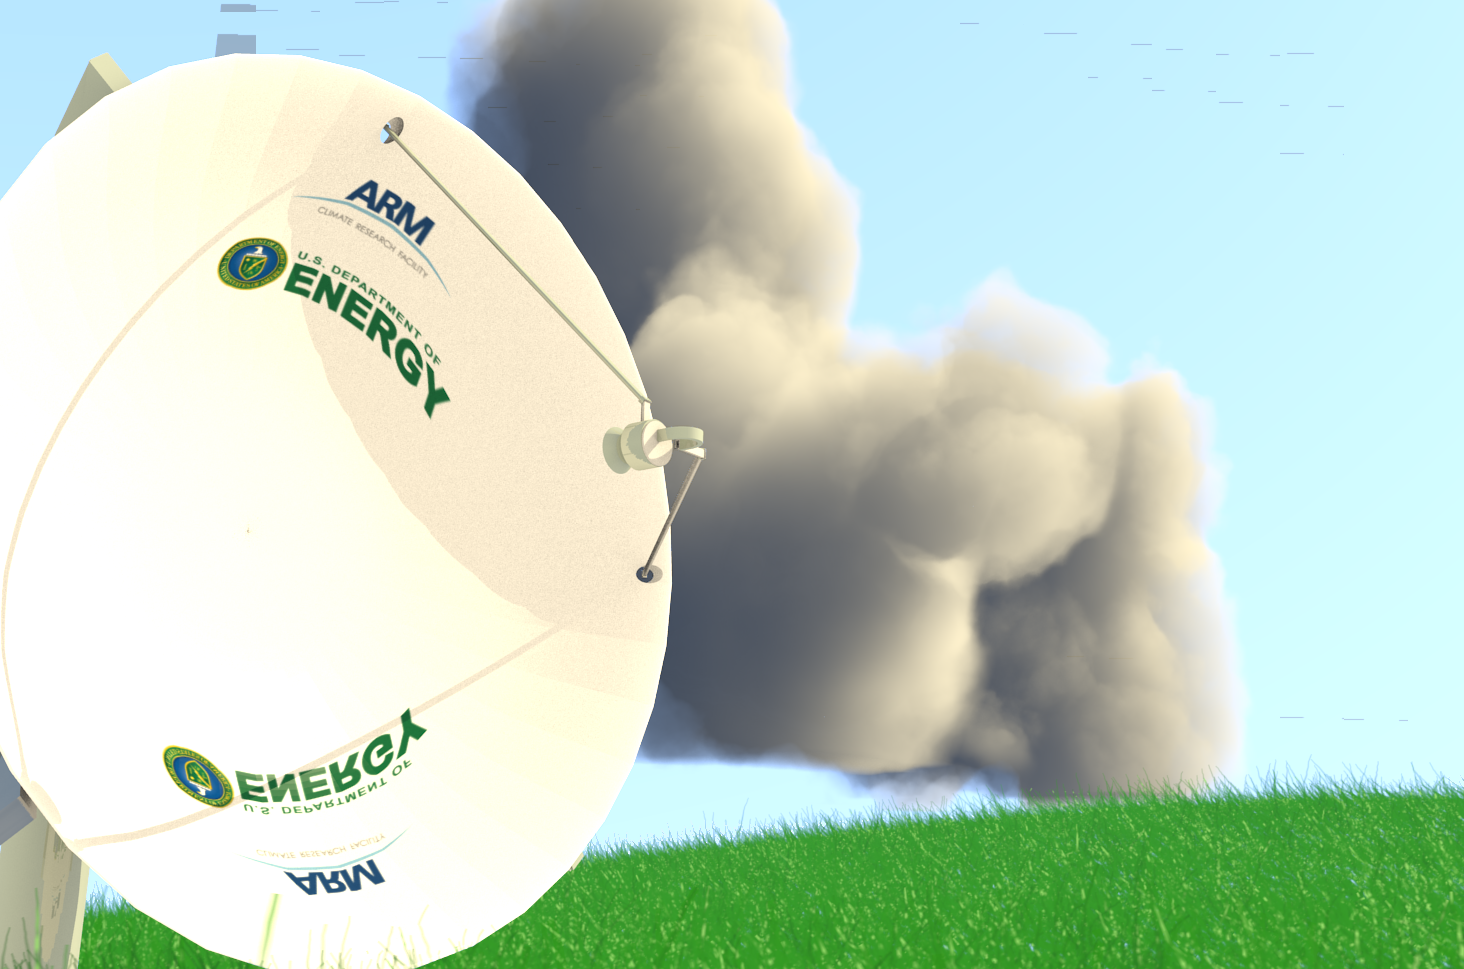
\includegraphics[height=\paperheight,width=\paperwidth]{figures/radar.png}};}


\title{\huge Architectures for Rainfall Property Estimation From Polarimetric Radar}
\author[Collis et al.]{Scott Collis, Scott Giangrande, Jonathan Helmus, and Silke Troemel}
\institute[Argonne]{Argonne National Laboratory Argonne, ILUnited States }
\date{\today}
\begin{document}
\begin{frame}{} 
 \begin{columns}[t]
    \begin{column}{.3\linewidth}
  \vfill
 
      \begin{block}{Introducton}
        \begin{columns}[t]
          \begin{column}{.5\linewidth}
        \begin{itemize}
        \item The Department of Energy's ARM Climate Research Facility operates a network of 5 and 3 cm scanning radar systems.
        \item Fixed sites are at the Azores, Southern Great Plains of Oklahoma and the town of Barrow on the North Slope of Alaska                                %what
         \end{itemize}
         \end{column}
          \begin{column}{.5\linewidth}
           \vskip0ex
            %%%%%%%%%%%%%%%%%%%%%%%%%%%%%%%%%%%
            \centering    
           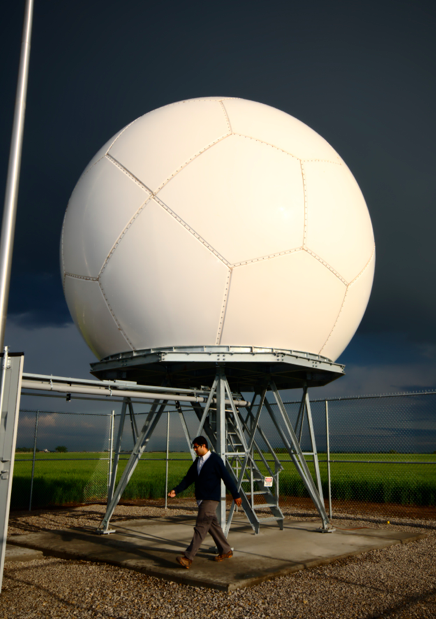
\includegraphics[width=0.4\linewidth]{figures/csapr.png}\\[1ex]            
          \end{column}
         \end{columns}
         \end{block}
       

     

    \end{column}
      \begin{column}{.3\linewidth}
  \vfill
 
      \begin{block}{Introduction}
        \begin{itemize}
        \item automatic sign language recognition system                                    %what
        \item \alert{necessary for communication} between deaf and
          hearing people
        \item \alert{continuous} sign language recognition,
          \alert{several} speakers, \alert{vision-based} approach, \alert{no
            special hardware}
        \item large vocabulary speech recognition (LVSR) system to
          obtain a textual representation of the signed
          sentences 
        \item evaluation of speech recognition techniques on \alert{publicly
          available sign language
          corpus}
        \end{itemize}
      \end{block}

 \begin{block}{Advective interpolation}

           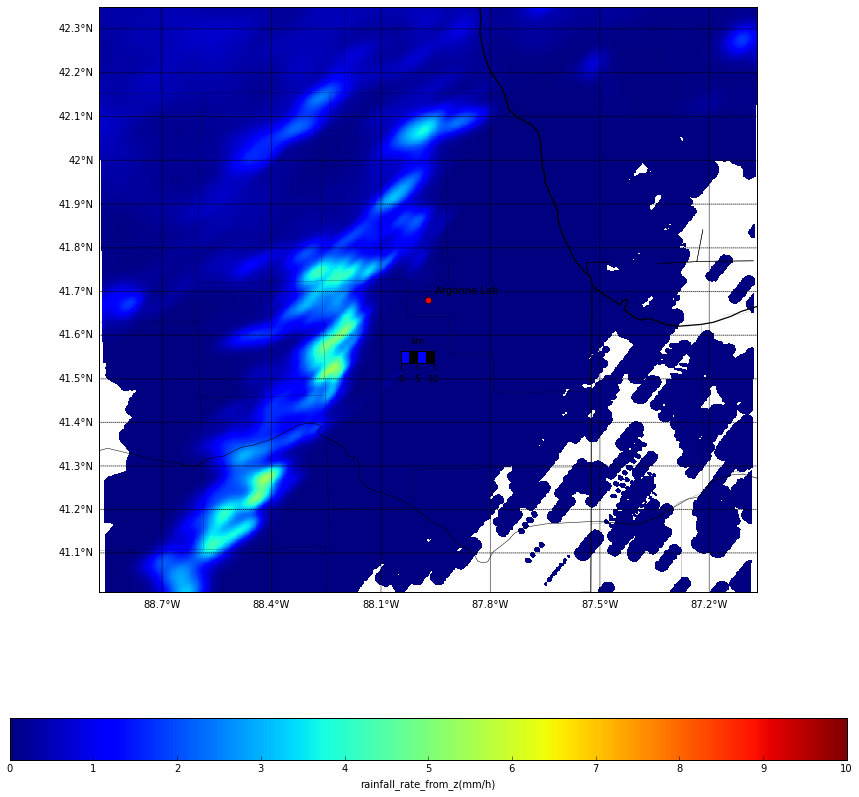
\includegraphics[width=0.7\linewidth]{figures/aggregate.png}\\[1ex]                      
  
      \end{block}
    \end{column}

  \begin{column}{.3\linewidth}
  \vfill
 
      \begin{block}{Introduction}
        \begin{itemize}
        \item automatic sign language recognition system                                    %what
        \item \alert{necessary for communication} between deaf and
          hearing people
        \item \alert{continuous} sign language recognition,
          \alert{several} speakers, \alert{vision-based} approach, \alert{no
            special hardware}
        \item large vocabulary speech recognition (LVSR) system to
          obtain a textual representation of the signed
          sentences 
        \item evaluation of speech recognition techniques on \alert{publicly
          available sign language
          corpus}
        \end{itemize}
      \end{block}

    \end{column}

  \end{columns}


  \vfill
\end{frame}
\end{document}


%%%%%%%%%%%%%%%%%%%%%%%%%%%%%%%%%%%%%%%%%%%%%%%%%%%%%%%%%%%%%%%%%%%%%%%%%%%%%%%%%%%%%%%%%%%%%%%%%%%%
%%% Local Variables: 
%%% mode: latex
%%% TeX-PDF-mode: t